\documentclass{article}%
\usepackage[T1]{fontenc}%
\usepackage[utf8]{inputenc}%
\usepackage{lmodern}%
\usepackage{textcomp}%
\usepackage{lastpage}%
\usepackage[head=40pt,margin=0.5in,bottom=0.6in]{geometry}%
\usepackage{graphicx}%
%
\title{\textbf{Vecinos protestan en El Paraíso por falta de servicios públicos}}%
\author{ERNESTO MENDEZ}%
\date{23/11/2018}%
%
\begin{document}%
\normalsize%
\maketitle%
\textbf{URL: }%
http://www.eluniversal.com/politica/26523/protestan{-}en{-}el{-}paraiso{-}por{-}falta{-}de{-}servicios{-}publicos\newline%
%
\textbf{Periodico: }%
EU, %
ID: %
26523, %
Seccion: %
politica\newline%
%
\textbf{Palabras Claves: }%
NO\_TIENE\newline%
%
\textbf{Derecho: }%
2.8%
, Otros Derechos: %
NO\_TIENE%
, Sub Derechos: %
2.8.1%
\newline%
%
\textbf{EP: }%
SI\newline%
\newline%
%
\textbf{\textit{Efectivos policiales se encuentran supervisando la manifestación que se desarrolla en la redoma La India, ubicada en El Paraíso}}%
\newline%
\newline%
%
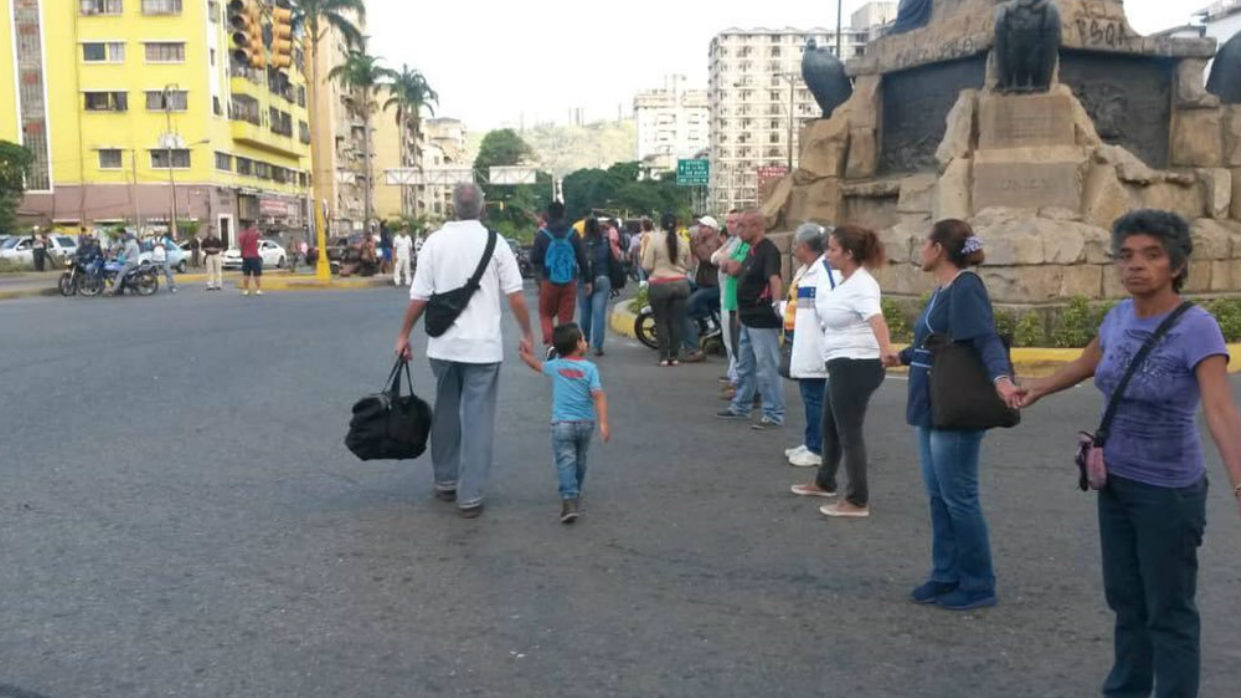
\includegraphics[width=300px]{127.jpg}%
\newline%
%
Caracas.{-} Vecinos manifiestan la mañana de este viernes en%
\newline%
%
la redoma La India, ubicada en el Paraíso, por fallas en el suministro de gas, luz y agua, así como deficiencias en la recolección de basura.%
\newline%
%
Usuarios reportaron a través de la red social Twitter que efectivos de seguridad se encuentran en el área supervisando la manifestación.%
\newline%
%
\end{document}